% Horizon penetrating coordinates (vs. Schwarzschild coordinates)
% for a black hole spacetime, with excision
% Author: Jonah Miller
\documentclass[tikz,border=0pt]{standalone}
\usepackage{tikz}
\usetikzlibrary{arrows}
\usetikzlibrary{arrows.meta}
\usetikzlibrary{decorations.markings}
\usepackage{pgfplots}
\usepackage{amsmath}
\usetikzlibrary{decorations.pathreplacing}
\usepackage{scalefnt}

\usepackage[utf8]{inputenc}

\usepgfplotslibrary{fillbetween}
\usepackage{lmodern}

%\tikzset{>={Latex[length=3mm]}}

\tikzstyle{mybox} = [draw=black,
    rectangle, inner sep=10pt, inner ysep=10pt]
\tikzstyle{fancytitle} =[fill=blue!30, text=black]

\begin{document}
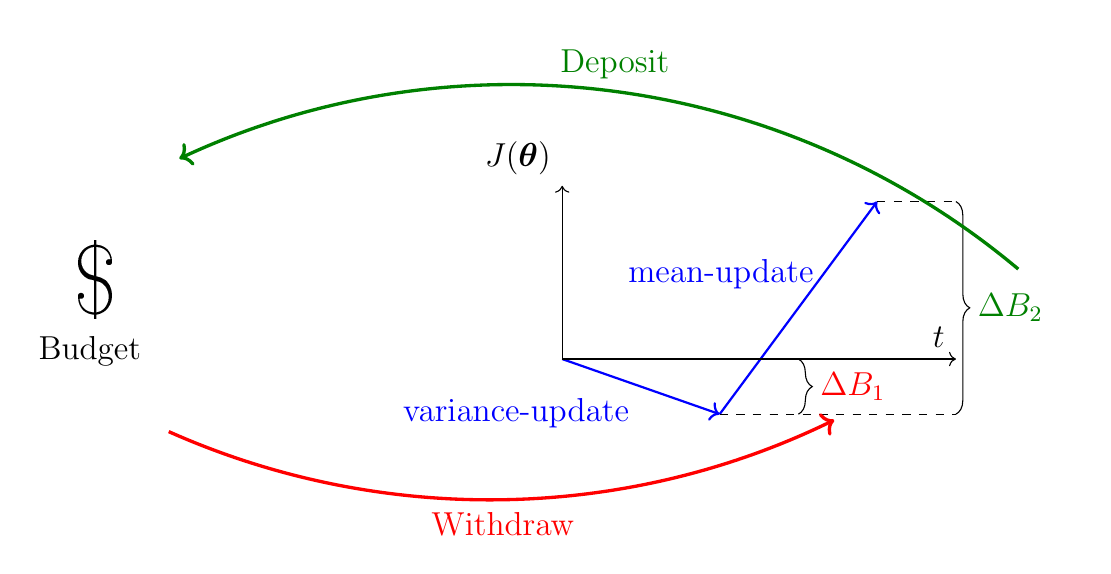
\begin{tikzpicture}[xscale=1]
\large

\draw[->, thick, blue] (0,0) -> (2,-0.7) node[midway,below left]{variance-update};
\draw[->, thick, blue] (2,-0.7) -- (4,2) node[midway,xshift=-28pt,yshift=12pt]{mean-update};% node[right,black]{$J(\boldsymbol{\theta}')$};

\draw[->] (0,0) -- (5,0) node[above left]{$t$};
\draw[->] (0,0) -- (0,2.2) node[above left]{$J(\boldsymbol{\theta})$};
%\draw [decorate,decoration={brace,amplitude=5pt,mirror,raise=0pt},xshift=0,yshift=0pt]
%(4.1,0) -- (4.1,1) node [black,midway,xshift=35pt,text width=1.5cm] 
%{\footnotesize greedy update};

%\draw[dashed] (4,2) -- (5.5,2);

\draw [decorate,decoration={brace,amplitude=5pt,mirror,raise=0pt},xshift=0,yshift=0pt]
(3,-0.7) -- (3,0) node(deltaone) [red,midway,xshift=25pt,text width=1.2cm] 
{$\Delta{B_1}$};
\draw[dashed] (2,-0.7) -- (5,-0.7);
\draw[dashed] (4,2) -- (5,2);

\draw [decorate,decoration={brace,amplitude=5pt,mirror,raise=0pt},xshift=0,yshift=0pt]
(5,-0.7) -- (5,2) node(deltatwo) [black!50!green,midway,xshift=25pt,text width=1.2cm] 
{$\Delta{B_2}$};
\draw[dashed] (2,-0.7) -- (3,-0.7);

%\node[right,yshift=10pt] at (4,2) {\begin{minipage}{4cm} $$  \begin{cases} w \gets w + \beta \nabla_w \mathcal{L}(\boldsymbol{\theta}) \\ \boldsymbol{v} \gets \boldsymbol{v} + \alpha \nabla_{\boldsymbol{v}}J(\boldsymbol{\theta}) \end{cases} $$ \end{minipage}};

%\node[right,xshift=5pt] at (4,1) {$\boldsymbol{v} \gets \boldsymbol{v} + \alpha \nabla_{\boldsymbol{v}}J(\boldsymbol{\theta})$};


\node [] (name) at (-6, 1) {\fontsize{120pt}{4pt} \selectfont \$};
\node[yshift=-7pt] at (name.south) {Budget};

\draw[black!50!green, very thick, ->] (deltatwo) ++(100:0.5)  arc (50:115:10) node[midway,above]{Deposit};
\draw[red, very thick, <-] (deltaone) ++ (-135:0.6) arc (-64:-114:10) node[midway,below]{Withdraw};

\end{tikzpicture}
\end{document}